
\begin{thanks}
博士论文写完了,二十一年的求学生活随之进入尾声。回首往事,我心中充满感激。
我有太多的人需要感谢。

首先,我要感谢我的导师、我最敬爱的袁老师。2006 年保研的时候,我其实并没有想
好要选择什么专业。六年前的那个下午,当我敲开袁老师的门,第一眼看到袁老师的
时候,就被老师的学者风度打动了。我依然清晰地记得那天袁老师与我面对面交谈的
情景,那是我第一次见到如此平易近人的老师。从那一刻起我就决定要做袁老师的学生。
如今,即将从袁老师这里毕业,我为当初的选择感到幸运。感谢袁老师五年来提供的宽松的研究
环境,让我可以研究自己喜欢的问题;感谢袁老师细心的指导,让我领略到优化之美,
领略到数学家思考问题的方式;感谢袁老师一直以来的鼓励和提携;感谢袁老师给我
出国访问的机会。我还要特别感谢袁老师在生活上对我的关心和照顾。五年里,袁老
师一直给予我父亲一般的关怀。2010 年夏天与袁老师在欧洲的三个月里,袁老师给我
做饭,带我旅游,让我懂得了什么叫师徒如父子。感谢袁老师一次又一次对我的教诲,
教给我生活的道理,分享给我人生的经验。是袁老师让我重新认识了生活。从袁老师
身上学到的每一点都是我最宝贵的财富。谢谢您,袁老师!

感谢我的师母张焱女士。感谢师母一直以来在生活上的关心和照顾。师母和袁老师让
我在北京感受到了家的温暖。我可能是被师母和袁老师叫到家里吃饭最多的学生。2010 
年夏天在欧洲的日子里,师母和袁老师像家人一样待我,让我度过了一段难忘的日子。
那段时间师母做的汤是世界上最好喝的汤。师母无论多忙,都会时常关心我的生活和
工作,让我心中多了一份前进的动力。

特别感谢袁老师的导师、英国皇家学会会员、美国科学院外籍院士、首届 Dantzig 奖
获得者、剑桥大学的 \mbox{M. J. D. Powell} 教授给我提供的指导和帮助。Powell 
教授对后辈的热情让我感动。每一次向 Powell 教授请教都让我获益匪浅。Powell 教
授提供了 \newuoa 算法的源代码和参考文献,这是我五年学习和研究中最重要的素材。

感谢德国拜罗伊特大学的 Klaus Schittkowski 教授和夫人。在 2010 年夏天我访问
拜罗伊特大学期间,教授和夫人给予了热情周到的接待,令我十分难忘。在拜罗伊特
的日子是这五年里我度过的最美好的时光。感谢洪堡基金资助我这次访问。本文
第\ref{chap:sobolev}章的部分内容就是在此次访问期间完成的。

感谢课题组的戴彧虹老师。戴老师在讨论班上的指点让我获益匪浅,这在论文里有直
接体现。戴老师豁达的生活态度和平易近人的风度永远值得我学习。感谢课题组的刘
歆老师。感谢刘老师五年以来像兄长一样的鼓励和帮助。

感谢课题组的夏勇博士、徐姿博士、牛凌峰博士、李在禾博士、付云姗博士、唐明筠
博士、程明厚博士、宫鲁津博士、郝春林博士、寇彩霞博士、费存林、
顾晓娟博士和李庆娜博士等师姐师兄们,感谢孙聪、张睿燕、姜波、Thanawath 
Niyamosoth、张文慧、刁瑞、刘田香、盛镇醴、崔春风、董乾和王树雄等师妹师弟和
同学们。感谢我的师兄丁晓东博士。我接触无导数优化算法就是从听师兄的报告开始的;
师兄在我研究的起步阶段提供了很多帮助,我使用的很多参考文献都是师兄提供的。
感谢与我同一级的王晓、刘亚锋和吴乐秦,和他们一起度过的五年,点点滴滴都值得
回忆。

Powell 教授、葡萄牙 Universidade de Coimbra 的 Lu\'{i}s Nunes Vicente 教授、
美国 Louisiana State University 的张洪超博士 (我的师兄) 以及李庆娜师姐、孙
聪师妹和姜波师弟审阅了我的第一篇论文 \cite{SobolevDFO} 并提出了宝贵的意见。
感谢他们对我的无私帮助。

感谢我在北京期间的室友张乔夫和张新雨、翟建梁两位师兄。我经常早出晚归,影响
了他们休息,感谢他们对我的包容。

感谢与我一同入所的何连花、梁珊、孙建青、王满、陈冲、陈耀、成杰、戴银云、黄
记祖、马云飞、伍泽东、肖俊敏和张乔夫。五年与他们一起走过我很荣幸。


感谢吴继萍老师、白英老师、丁如娟老师、樊建荣老师、刘颖老师、钱莹老师、张纪
平老师、魏敏老师、关华老师、王璐璐老师、邵欣老师和尹永华老师五年期间对我的
帮助。

感谢我的母校、我深怀眷恋的吉林大学。人生最美好的四年能在吉大度过,我很幸运。
特别感谢吉林大学数学学院的老师们。感谢谢敬然老师。谢老师并不认识我,但是是
他的引导让我走入了数学的美妙世界。感谢马富明老师。马老师对学生的爱护和提携
是我学习的榜样。感谢李永海老师。李老师对学生的真诚让人感动。感谢纪友清老师。
纪老师讲授的泛函分析塑造了我的思维方式。感谢大学四年所有教过我的老师。从他
们身上,我学到了很多很多。

特别感谢我的启蒙老师夏翠苓女士。回首漫漫求学路,我取得的每一点进步都深深地
植根于您二十年前的教诲。

感谢中学和大学里与我一起笑过、哭过、奋斗过的兄弟们。有你们在,我活得很踏实。
特别感谢王振宇、张明涛、石胜坤和张旭升。五年里,你们一直是我在北京最可靠的
后盾。

最后,我要感谢我的家人。感谢我深爱的父亲母亲。做你们的儿子是我此生最幸运的
事情;是你们教会我,诚实的劳动是获得成功的唯一方法;在我 失落的时候,你们是
我内心最大的慰藉;在我遭受挫折的时候,想到你们我总能找回前进的勇气。谢谢你
们,我爱你们!感谢我的哥哥和嫂子,感谢他们一直以来对我的照顾。若没有哥哥当
初的建议,我不会报考吉林大学数学学院,这是改变我一生的事情。

%本文完成之后的第十天 (2012 年 4 月 17 日,壬辰年三月廿七) 是母亲六十岁生日。
本文完成之后的第十天 (壬辰年三月廿七) 是母亲六十岁生日。
我谨以此文作为献给母亲的生日礼物,祝母亲健康、平安。

%\begin{flushright}
%    {\kaishu{张在坤}}\\
%    2012 年 4 月 7 日\\
%    于北京保福寺
%\end{flushright}
\begin{flushright}
    {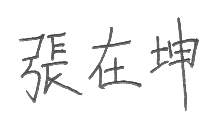
\includegraphics[width=0.16\textwidth]{zzk.eps}}\\
    2012 年 4 月 7 日\\
    于北京保福寺
\end{flushright}
\end{thanks}
